You can start JavaFX \gdauts{} via a configuration, but not via \bxname{autrun}.


\subsubsection{Configuring a Java \gdaut{} to be started from the \ite{}}
\index{Add!AUT Configuration}
\index{AUT Configuration!Add}
\index{Edit!AUT Configuration}
\index{AUT Configuration!Edit}
\index{Working Directory}
\index{CmdLineParameter}
\index{Environment}
\index{AUT!Configuration}
\index{Configuration!AUT}
\index{Activation}
\index{Application activation}
\index{AUT ID}
\label{TasksConfigureFXAUT}

The \gdaut{} configuration dialog for Java FX has three different levels of detail: basic, advanced and expert. 

See the sections below for information on the different levels. 

\subsubsection{Basic JavaFX \gdaut{} configuration}

You can use the basic setting to configure your \gdaut{} if it can be started by an executable file (e.g. .bat, .exe, .cmd, .sh etc.). 
If your \gdaut{} is a JAR, then you can also use the executable file field to enter the Java executable (i.e. java or java.exe) and then enter the path to the JAR in the AUT Arguments field in the advanced configuration \bxpref{AdvancedAUTConfig}.

\bxtipp{You must be using a Java 8 JRE to be able to start JavaFX \gdauts{}.}

\begin{enumerate}
\item Enter the basic configuration details as described earlier \bxpref{TasksBasicConfigurationInfo}.
\item Enter the executable file name in the \bxname{Executable File Name} field. This path can be relative if you define a working directory \bxpref{AdvancedAUTConfig}).
  
\end{enumerate}
For information on the advanced properties for the \gdaut{} configuration, see the next section \bxpref{AdvancedAUTConfig}. 


\subsubsection{Advanced JavaFX \gdaut{} configuration}
\label{AdvancedAUTConfig}

The advanced configuration dialog lets you create a working directory for your \gdaut{}, and add command-line arguments needed to start the \gdaut{}. If you entered a Java executable as the executable file name in the basic configuration, then you can enter \bxshell{-jar <JARFILE>} in the AUT Arguments field (\bxfigref{autconfigjavafxwithjar}).

\begin{figure}[h]
\begin{center}
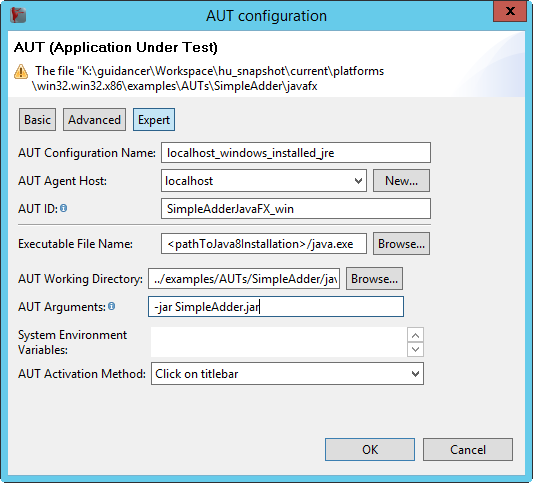
\includegraphics[width=7cm]{Tasks/AUTs/PS/javafxconfigwithjar}
\caption{Example JavaFX \gdaut{} configuration}
\label{autconfigjavafxwithjar}
\end{center}
\end{figure}

For information on the expert properties for the \gdaut{} configuration, see the next section \bxpref{ExpertAUTConfig}. 

\subsubsection{Expert JavaFX \gdaut{} configuration}
\label{ExpertAUTConfig}
You can use the expert dialog to configure more detailed information about how the \gdaut{} should be started. 


\begin{enumerate}
\item Enter any required \bxname{System Environment Variables}, in the
format \bxcaption{<VARNAME>=<value>}, i.e. \bxcaption{PATH=C:$\backslash$}. 
Separate each variable with a new line by pressing \bxkey{Enter}.

\bxwarn{Please be advised that ''embedding'' the contents of one
variable into another is not supported at this time. That is,
if you have a variable named \texttt{FOO} whose value is
\bxcaption{abc}, and set the value of a second
variable \texttt{BAR} to \bxcaption{\%FOO\%def}, the second variable will
\emph{not} contain \bxcaption{abcdef}, but rather the exact text
\bxcaption{\%FOO\%def}, without evaluating it.}


\item Select an activation method for your \gdaut{}. More information on \gdaut{} activation is available in the previous section \bxpref{TasksAUTActivation}.


\end{enumerate}
